\newpage
\section{Functions}

\subsection{Functions identification}

In a first approach, we can identify seven main functions:

\begin{enumerate}
    \item \textbf{Expose api}: the system will expose a public api and prevent access to any private api.
    \item \textbf{Protect git}: the system will authenticate and authorize users to perform git or git-lfs commands.
    \item \textbf{Execute git commands}: the system will execute git commands on behalf of the user, and actually store the repositories in a centralized way.
    \item \textbf{Handle locks}: the system will provide the locking mechanism defined by git-lfs.
    \item \textbf{Protect LFS api}: the system will manage git-lfs requests, mainly verifying that user can upload/download objects
    \item \textbf{Store large objects}: the system will store and retrieve the objects
    \item \textbf{Manage repositories and users}: the system will provide interfaces and mechanisms to manage repositories and users
\end{enumerate}

If we break down these functions one level down, we can identify the sub-functions described by figure \ref{fig:functions}.

\begin{figure}[h]
    \centering
    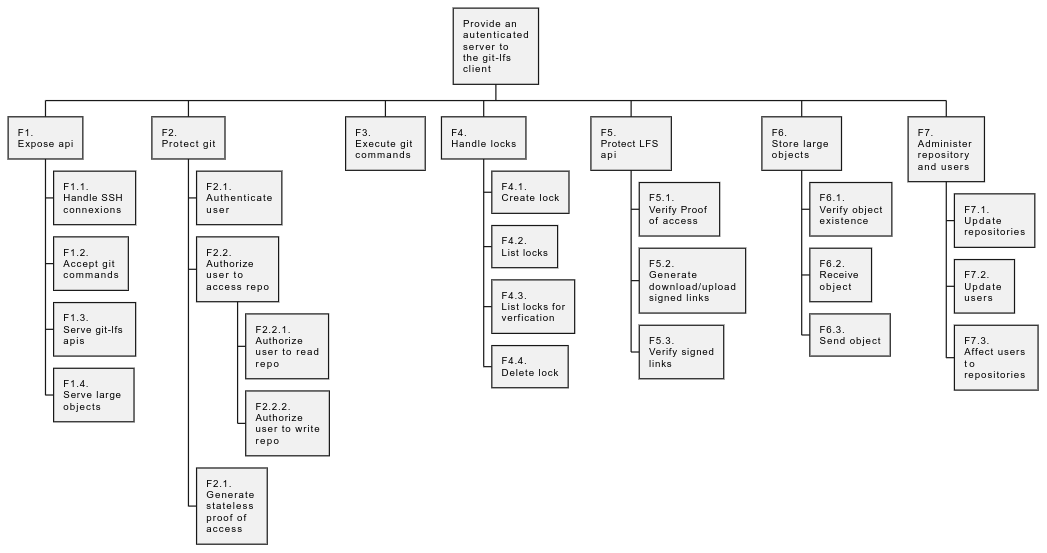
\includegraphics[width=\textwidth]{iteration_00/diagrams/functions.png}
    \caption{Functions}
    \label{fig:functions}
\end{figure}

\subsection{Functions satisfying requirements}

These functions satisfy the requirements of table \ref{tab:requirements}, as shown in the following table:

\begin{longtable}{|p{0.05\textwidth}|p{0.75\textwidth}|p{0.15\textwidth}|}
    \hline
    id  & description                                                                                                          & Satisfied by function \\ \hline
    \endfirsthead
    %
    \endhead
    %
    R1  & The system shall serve all regular git commands (clone, push, pull, etc.).                                           & F3                    \\ \hline
    R2  & The system shall allow for SSH git authentication.                                                                   & F1.1                  \\ \hline
    R3  & The system shall allow for per-repository access control, including read and write access.                           & F7                    \\ \hline
    R4  & The system shall implement the git-lfs batch/objects API.                                                            & F5, F6                \\ \hline
    R5  & The system shall implement the git-lfs locks API.                                                                    & F4                    \\ \hline
    R6  & The system shall store LFS files in a separate storage location.                                                     & F6                    \\ \hline
    R7  & Components of the system shall be reusable in other systems.                                                         & -                     \\ \hline
    R8  & Only the lock API, the batch API, and the git commands shall be exposed to the outside.                              & F1.2, F1.3, F1.4      \\ \hline
    R9  & The system shall be configurable by a single administrator actor (other authorized system or actual person).         & F7                    \\ \hline
    R10 & The authorization systems shall not share state between the git server and the git-lfs server or the storage server. & F2.3, F5              \\ \hline
    R11 & A single implementation of the system shall be implemented by the end of September 2023                              &                       \\ \hline
\end{longtable}

\subsection{Detailed interactions}

As a (too complex) overview, the functions interact with each other as shown in figure \ref{fig:functions_detail}. To break down the complexity, let's consider a few projections of this model.

\begin{figure}[h]
    \centering
    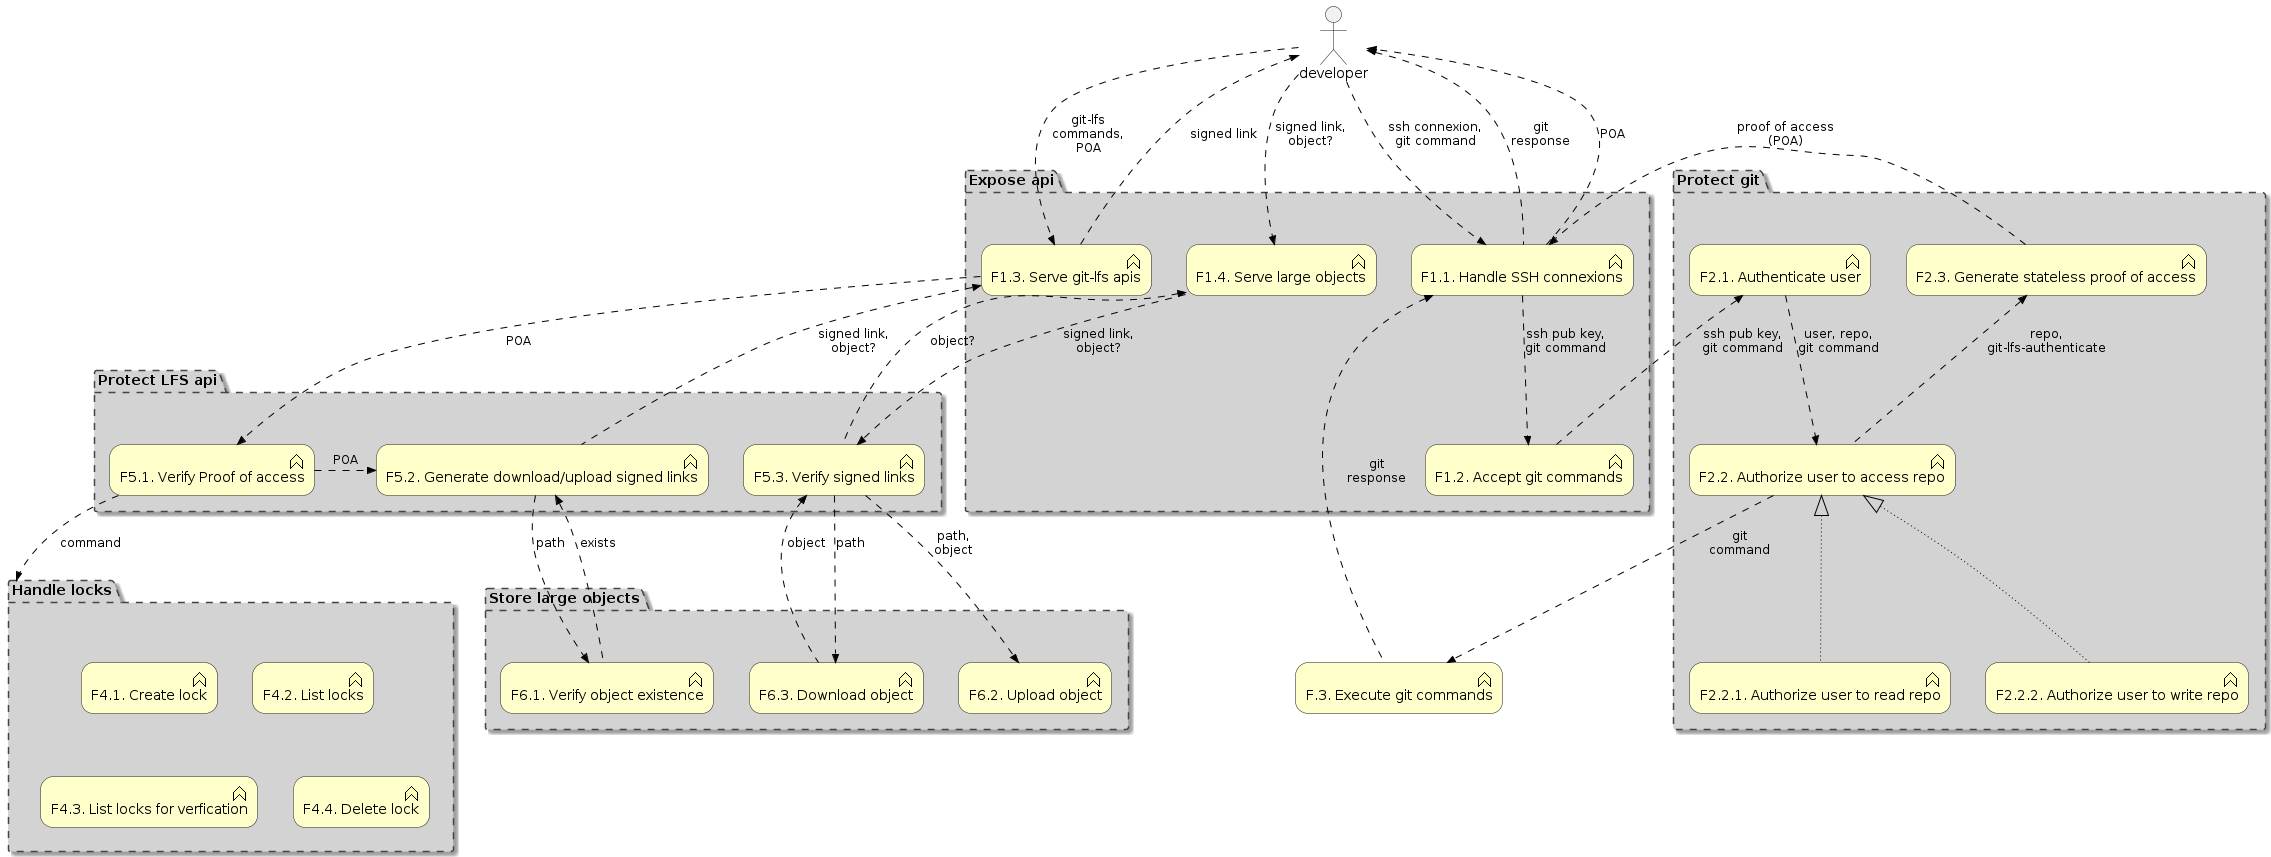
\includegraphics[width=\textwidth]{iteration_00/diagrams/detailed_flow.png}
    \caption{Details of functions interactions}
    \label{fig:functions_detail}
\end{figure}

\subsection{Interactions of first level functions}

At first level, the developer run git commands and get responses. Down, either we go to the git protection functions, and the git functions, or we go to the git-lfs related functions. This separation satisfies R10, as only the stateless proof of access (POA) is shared. User request one to the "git-related" functions, and use it into the "git-lfs" functions. The data flows are shown in figure \ref{fig:functions_overview}

\begin{figure}[h]
    \centering
    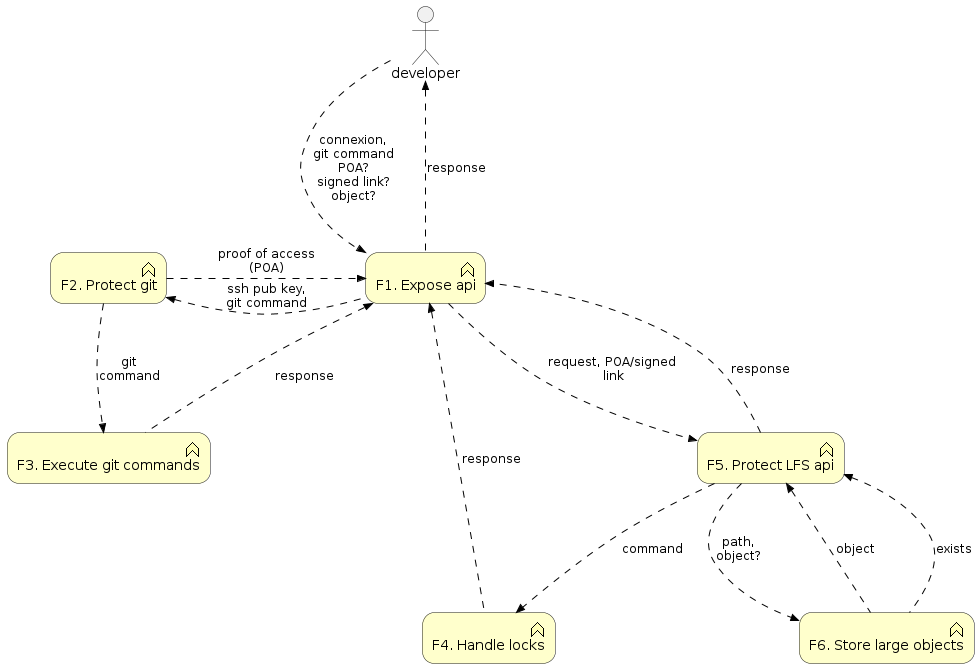
\includegraphics[width=\textwidth]{iteration_00/diagrams/overwiew_flow.png}
    \caption{Overview}
    \label{fig:functions_overview}
\end{figure}

\newpage
\subsection{Regular git flow interactions}

When developer run regular git commands, (no lfs), his SSH connexion must be handled, and then we are ready to accept git commands. But before running them, we shall ensure the uses is allowed to perform them, using the function F2. Then, the git command can be executed and the result be returned to the user via the SSH channel. The whole interaction is shown in figure \ref{fig:simple_git_flow}

\begin{figure}[ht]
    \centering
    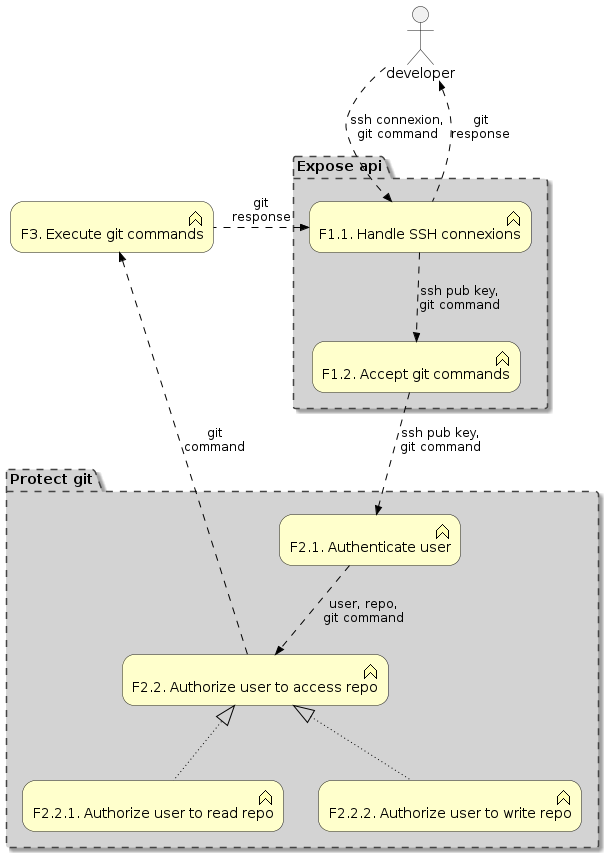
\includegraphics[width=0.6\textwidth]{iteration_00/diagrams/simple_git_flow.png}
    \caption{Simple git flow}
    \label{fig:simple_git_flow}
\end{figure}

\newpage
\subsection{Stateless proof of access flow}

When developer run lfs git commands, he first need to get authenticated. As the lfs functions are unable to access the authorization state of the user, he first need to acquire a proof that he can perform an LFS action. So user first connect through SSH to the authentication server, get a proof of access, and then can use it. The POA acquisition flow is shown in figure \ref{fig:POA_flow}

\begin{figure}[ht]
    \centering
    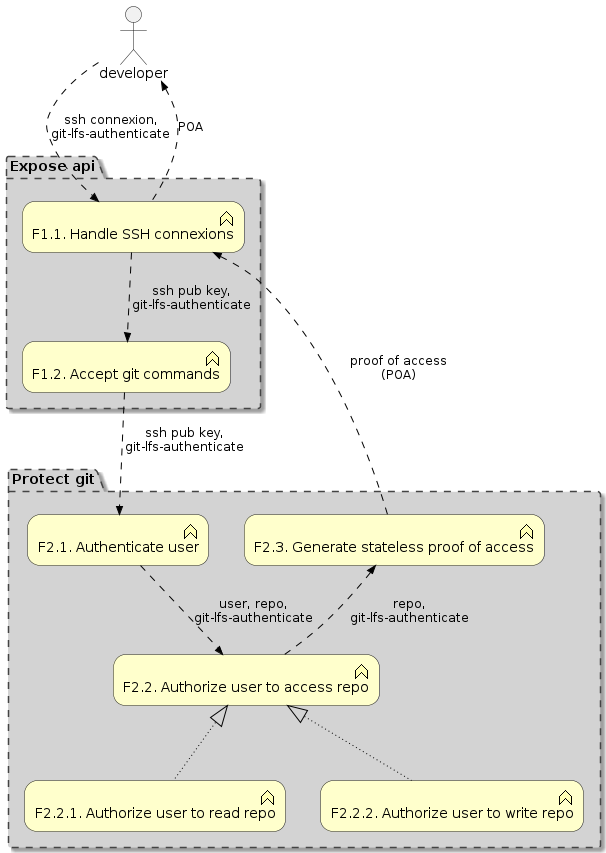
\includegraphics[width=0.6\textwidth]{iteration_00/diagrams/POA_flow.png}
    \caption{POA acquisition flow}
    \label{fig:POA_flow}
\end{figure}

\newpage
\subsection{LFS API flow}

After the user got a POA, he can use it to connect to the LFS api functions, that first verify the POA, and the serve files, locks... The files are also served indirectly, with a stateless signed link, so between requests, no state is saved in the LFS server, even if user can't download all files at once. As defined in the LFS api, the user first request a list of files, get a list of signed links, and the get them one by one. The functions involved in this use of the LFS api are shown in figure \ref{fig:signed_link_flow}

\begin{figure}[ht]
    \centering
    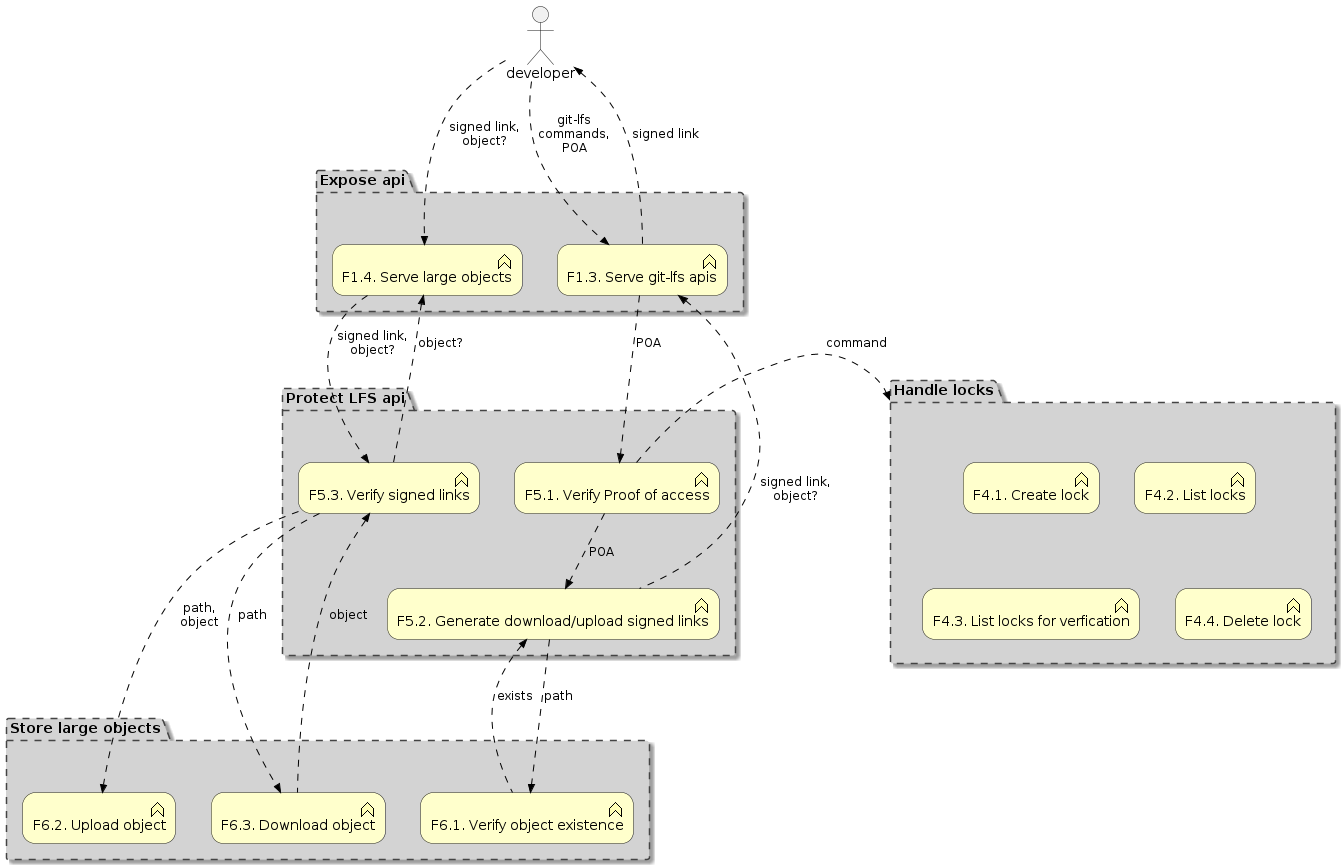
\includegraphics[width=\textwidth]{iteration_00/diagrams/signed_link_flow.png}
    \caption{LFS API flow}
    \label{fig:signed_link_flow}
\end{figure}
